\documentclass[a4,12pt]{book}

\usepackage{template}

% Parallelepiped definitions
\usetikzlibrary{quotes,arrows.meta}


\begin{document}

\chapter{Começando a falar sobre frações }

\section*{EXPLORANDO O ASSUNTO }

\subsection{Atividade}

Três irmãos vão repartir uma barra de chocolate. Um deles sugere a seguinte divisão: 

\begin{imagem*}[breakable]{}{}   - FIGURA ARTÍSTICA   
  
Na imagem devem estar 3 irmãos, aparentando idades diferentes (um deles pode ser cadeirante, por exemplo), observando uma única barra de chocolate retangular (preferencialemnte,   {\bf imagem tridimensional sem subdivisões}  ) repartida em três partes com tamanhos diferentes. Por exemplo:  
  
    \includegraphics[width=180pt, keepaspectratio]{../../livro/media/cap1/secoes/licao1_1.png}  
  
\end{imagem*}

\begin{enumerate} [\quad a)] %s
  \item     Você concorda com essa divisão? Explique.
  \item     Com essa divisão, os três irmãos receberão a mesma quantidade de chocolate?
  \item     Use a imagem a seguir para mostrar uma divisão da barra de chocolate que permita que os 3 irmãos recebam quantidades iguais de chocolate. 
\begin{imagem*}[breakable]{}{}    - FIGURA ARTÍSTICA - Inserir imagem da mesma barra retangular de chocolate da ilustração anterior sem qualquer partição sugerida. Apenas a imagem da barra de chocolate. Não há necessidade de ilustrar os irmãos.\end{imagem*}
  \item     Considerando a divisão da barra de chocolate em 3 partes iguais, como você nomearia a quantidade de chocolate que cada irmão receberia? 
\end{enumerate} %s

\subsection{Atividade}
Três pizzas inteiras, de mesmo tamanho, foram repartidas entre as crianças de uma turma. Para isso, a turma foi dividida em três grupos com quatro crianças cada. Veja como cada grupo repartiu a sua pizza.

\begin{imagem*}[breakable]{}{}    - FIGURA ARTÍSTICA - A imagem deve conter 3 GRUPOS com 4 CRIANÇAS cada (Diversificar as características físicas das crianças). Cada um dos grupos deve estar observando uma pizza. Colocar duas das crianças do grupo 3 com feições   ``contrariadas''  . As pizzas devem ter mesmos tamanho e formato. As pizzas devem estar repartidas de três maneiras diferentes, como indicado nas imagens a seguir: Grupo 1, Grupo 2 e Grupo 3:   
    \includegraphics[width=300pt, keepaspectratio]{../../livro/media/cap1/secoes/licao1_atv2.png}  
  ilustração: Cambrainha  
\end{imagem*}

\begin{enumerate} [\quad a)] %d
  \item     Cada um dos três grupos repartiu a sua pizza na mesma quantidade de fatias que os outros grupos?
  \item     Dessa maneira, todas as crianças da turma receberam a mesma quantidade de pizza?
  \item     Em algum dos grupos as 4 crianças receberam a mesma quantidade de pizza? Se sim, em qual? Considerando a pizza inteira, como você nomearia cada uma das fatias de pizza desse grupo? 
\end{enumerate} %d

\subsection{Atividade}

Alice quer enfeitar a sala de aula e pretende prender os enfeites utilizando pedaços de barbante. Para isso, quer cortar o barbante em pedaços iguais, para que os enfeites fiquem todos na mesma altura. Ajude Alice a cortar o barbante.

\begin{imagem*}[breakable]{}{}    - FIGURA ARTÍSTICA - Incluir imagem de um pedaço de barbante e de 4 estrelas congruentes, como ilustrado a seguir:  
  Alice é uma menina morena de rabo de cavalo. Ela será um personagem frequente deste livro.  
  {\bf NÃO REPRODUZIR A IMAGEM DO PENSAMENTO DE ALICE}  , mas colocar uma em que apareça uma da estrelas pendurada em um pedaço de barbante.   
  
    \includegraphics[width=180pt, keepaspectratio]{../../livro/media//cap1/secoes/alice_barbante_estrelas.jpg}  
\end{imagem*}

\begin{imagem*}[breakable]{}{}   - FIGURA ARTÍSTICA -  
  \begin{nota*}[breakable]{}{}         
    INCLUIR PÁGINA DE REPRODUÇÃO COM apenas 1 ESTRELA com aproximadamente 15 cm de altura para ser recortada.    
  \end{nota*}  
\end{imagem*}

\section*{ORGANIZANDO AS IDEIAS }

Nas atividades anteriores, as quantidades registradas exigiram a partição de uma unidade. Por exemplo, para obter um terço de uma barra de chocolate foi necessário partir a barra de chocolate. Já para obter um quarto de pizza, foi necessário partir a pizza. Outros exemplos aparecem no dia a dia: ``Comprei meio metro de tecido'' ou ``Gastei um terço da minha borracha''.

A barra de chocolate, a pizza e o pedaço de barbante foram partidos em partes iguais. 
Em cada um dos casos, o que foi repartido é chamado {\bf unidade}. Cada uma das partes em que essas unidades foram repartidas igualmente é uma {\bf fração da unidade}. Assim, por exemplo, um quarto de uma pizza é uma fração da pizza e a pizza é unidade. Se a unidade for o pedaço de barbante, um quarto do pedaço de barbante será uma fração do pedaço de barbante.

\begin{imagem*}[breakable]{}{}   - FIGURA ARTÍSTICA -  
  {\bf Imagem de uma pizza e de um pedaço de barbante, cada um dividido em 4 partes.}  
\end{imagem*}

O nome dado à fração da unidade depende da quantidade de partes em que a unidade é dividida. 

Ao dividir uma unidade qualquer em duas partes iguais, ou ao meio, cada uma das partes é chamada de {\it um meio} ou {\it a metade} da unidade. 

Por exemplo, se uma barra de chocolate é repartida igualmente entre dois amigos, a quantidade que caberá a cada um dos amigos é {\it um meio} da barra de chocolate (ou {\it metade} da barra). Nesse exemplo, a unidade é a barra de chocolate.

\begin{imagem*}[breakable]{}{}   - FIGURA ARTÍSTICA - INCLUIR IMAGENS ILUSTRATIVA de metade   
  {\bf Imagem de duas crianças a barra de chocolate em que a metade é identificada}  
\end{imagem*}

Ao dividir uma unidade em três partes iguais, cada uma das partes é chamada de {\it um terço} ou {\it a terça parte} da unidade. 

Por exemplo, se, em uma receita de bolo, é necessário acrescentar {\it um terço} de um litro de leite. Isso significa que, para colocar a quantidade correta de leite na receita, é preciso repartir o litro de leite em três partes iguais e usar apenas uma dessas partes, que é {\it um terço} do litro de leite. Nesse caso, a unidade é um litro de leite.

\begin{imagem*}[breakable]{}{}   - FIGURA ARTÍSTICA - INCLUIR IMAGEM ILUSTRATIVA de terço   
  {\bf Sobre uma mesa, uma garrafa cilindrica cheia de leite e três garrafas iguais ao lado, cada uma com 1/3 da capacidade prennchida.}  
  
  Por exemplo:   
    \includegraphics[width=60pt, keepaspectratio]{../../livro/media//cap1/secoes/litro_de_leite.jpg}  
    \includegraphics[width=60pt, keepaspectratio]{../../livro/media//cap1/secoes/um_terco_de_litro_de_leite.jpg}  
  
\end{imagem*}

Ao dividir uma unidade em quatro partes iguais, cada uma das partes é chamada de {\it um quarto} ou {\it quarta parte} da unidade. 

Por exemplo,
A parte colorida da figura é um quarto da figura. Neste caso, a figura é a unidade.

\begin{imagem*}[breakable]{}{}   - FIGURA ARTÍSTICA - INCLUIR IMAGEM ILUSTRATIVA de quartos  
    \includegraphics[width=120pt, keepaspectratio]{../../livro/media//cap1/secoes/quartos_conexoes.jpg}  
   \end{imagem*}

Da mesma forma, ao dividir uma unidade em cinco partes iguais, cada uma das partes é chamada de {\it um quinto} ou {\it quinta parte} da unidade.

Por exemplo,
{\it um quinto} de todo ouro pesado nas Casas de Fundição no Brasil era pago em impostos à Coroa Portuguesa. Desta forma, a quantidade de ouro pago em impostos à Coroa Portuguesa era igual a {\it um quinto} ou a {\it quinta parte} do ouro pesado nas Casas de Fundição no Brasil.

\begin{imagem*}[breakable]{}{}   - FIGURA ARTÍSTICA - INCLUIR IMAGEM ILUSTRATIVA de quintos   
  {\bf Um homem entregando um saco de ouro a um rei e ficando com outros 4 sacos}  
\end{imagem*}

\section*{MÃO NA MASSA }

\subsection{Atividade}

\begin{enumerate} [\quad a)] %s
  \item     Quais dos retângulos a seguir foram repartidos em     {\it quartos}    ?     \mbox{} \newline      
 %\vspace{0.2cm}
 
 \begin{tikzpicture}[scale=5]
  \draw[attention] (0,0) rectangle (1,6);
  \draw[attention] (1,0) rectangle (2,6);
  \draw[attention] (2,0) rectangle (3,6);
  \draw[attention] (3,0) rectangle (4,6);
  \draw[common] (5,0) rectangle (9,3);
  \draw[common] (5,0) rectangle (9,6);
  \draw[common] (5,0) -- (9,3);
  \draw[common] (5,3) -- (9,6);
  \draw[special] (10,0) rectangle (14,3);
  \draw[special] (10,3) rectangle (14,6);
  \draw[special] (12,0) -- (12,3);
  \draw[special] (10,4.5) -- (14,4.5);
  \draw[dark] (15,0) rectangle (19,3);
  \draw[dark] (15,3) rectangle (19,6);
  \draw[dark] (15,1.5) -- (19,1.5);
  \draw[dark] (15,3) -- (19,6);
\end{tikzpicture}
\vspace{0.2cm}

\begin{tikzpicture}[scale=5]
  \draw[attention] (0,0) rectangle (4,1.5);
  \draw[attention] (0,1.5) rectangle (4,3);
  \draw[attention] (0,3) rectangle (4,4.5);
  \draw[attention] (0,4.5) rectangle (4,6);
  \draw[common] (5,0) rectangle (9,3);
  \draw[common] (5,0) rectangle (9,6);
  \draw[common] (7,0) -- (7,6);
  \draw[special] (10,0) rectangle (14,3);
  \draw[special] (10,3) rectangle (14,6);
  \draw[special] (12,0) -- (12,3);
  \draw[special] (10,3) -- (14,6);
  \draw[dark] (15,0) rectangle (19,3);
  \draw[dark] (15,3) rectangle (19,6);
  \draw[dark] (15,0) -- (19,3);
  \draw[dark] (19,3) -- (15,6);
\end{tikzpicture}
  
  \item     Desenhe um retângulo e faça uma partição desse retângulo em quatro partes que não sejam todas quartos.
\end{enumerate}

\begin{refletindo*}[breakable]{}{}  
  Quando se diz que uma unidade é repartida em meios, terços, quartos, quintos, etc., a unidade foi repartida em 2, 3, 4, 5, etc., partes iguais.  
  Assim como no dia a dia, neste livro o termo   ``partes iguais''   quer dizer   ``partes com a mesma quantidade''  , mesmo que a unidade não esteja dividida em partes de mesma forma.  
  Na atividade anterior, se os retângulos representassem, por exemplo, bolos, as quatro partes em que foram divididos os retângulos representariam quantidades iguais de bolo.   
  Em alguns retângulos as partes não têm a mesma forma.  
  Veja alguns exemplos curiosos em que as   ``partes iguais''   podem gerar confusão.  
  
  \begin{imagem*}[breakable]{}{}     FIGURA ARTÍSTICA    
    
    {\bf Quadrinho 1:}     Uma menina chega ao balcão de uma loja em que há uma pizza inteira:     
    
    Menina: Bom dia! Metade desta pizza, por favor.     
    
    Vendedor: É pra já, vou cortar para você!    
    
        \includegraphics[width=120pt, keepaspectratio]{../../livro/media//cap1/secoes/193px-pepperoni_pizza_2_.png}    
    ilustração: Pogrebnoj-Alexandroff    
    
    {\bf Quadrinho 2:}     O vendedor entrega a metade da pizza à menina. Mas ao invés de simplesmente cortada ao meio com um segmento de reta, a pizza foi dividida com um S. A menina olhando com ar espantado.     
    
        \includegraphics[width=120pt, keepaspectratio]{../../livro/media//cap1/secoes/pizza_yinyang.png}    
  \end{imagem*}  
  
  \begin{imagem*}[breakable]{}{}     FIGURA ARTÍSTICA    
    
    Dois amigos terminam de preparar uma torta na cozinha de sua casa e olhando empolgados para a torta diante deles na mesa.    
    
    {\bf Quadrinho 1:}         
    
    Menino 1:  Terminamos! Mas agora preciso ir que minha mãe está me esperando. Vou avisá-la que já estou indo.    
    
        \includegraphics[width=120pt, keepaspectratio]{../../livro/media//cap1/secoes/torta_abacaxi1.jpg}    
    
    ilustração: Kimberly Vardeman    
    
    Menino 2: Certo, vou dividir meio a meio para você levar a sua metade com você.    
    
    {\bf Quadrinho 2:}    
    O menino 1 está falando ao telefone afastado e o menino 2 está cortando a torta ao meio. Mas ele está fazendo um corte na horizontal para ficar com todo a cobertura para si.    
  \end{imagem*}  
\end{refletindo*}

\subsection{Atividade}

Em cinco das figuras a seguir a parte em vermelho é um terço da figura. Identifique essas figuras.

\begin{center}
\begin{tabular}{ccc}
a)
\parbox[t][3cm][c]{5cm}{
\begin{tikzpicture}[scale=0.7]
      \draw[attention] (90:2 cm)  -- (210:2 cm);
      \draw (210:2 cm)  -- (330:2 cm);
      \draw[attention] (330:2 cm) -- (90:2 cm);      
\end{tikzpicture}
}
& \quad \quad  &
f)
\parbox[t][3cm][c]{5cm}{
\begin{tikzpicture}[scale=0.7]
\foreach \x in {0,60,...,300}{
      \draw (\x:2 cm)  -- (\x + 60:2 cm);}
      \draw (0,0)  -- (60:2 cm);
      \draw (0,0)  -- (180:2 cm);
      \fill[attention] (0,0) -- (60:2 cm) -- (120:2 cm) -- (180:2 cm) -- (0,0);
      \fill[common] (0,0) -- (60:2 cm) -- (0:2 cm) -- (300:2 cm) -- (240:2 cm) -- (180:2 cm) -- (0,0);
      \draw (0,0)  -- (300:2 cm);
\end{tikzpicture}
}
\\

b)
\parbox[t][3cm][c]{5cm}{
\begin{tikzpicture}[scale=6]
      \draw (0,0) rectangle (4,3);
      \draw (0.5,0.5) rectangle (3.5,2.5);
      \fill[common] (0,0) -- (0.5,0.5) -- (3.5,0.5) -- (3.5,2.5) -- (4,3) -- (4,0)--cycle;
      \fill[attention] (0,0) -- (0.5,0.5) -- (0.5,2.5) -- (3.5,2.5) -- (4,3) -- (0,3)--cycle;
\end{tikzpicture}
}
& &

g)
\parbox[t][3cm][c]{5cm}{
\begin{tikzpicture}[scale=4]
      \draw[attention] (0,3) -- (3,0);
      \draw[attention] (3,0) -- (6,3);
      \draw (6,3) -- (9,0);      
\end{tikzpicture}
}
\\

c)
\parbox[t][3cm][c]{5cm}{
\begin{tikzpicture}[scale=4]
      \draw (0,3) -- (3,0);
      \draw[attention] (3,0) -- (6,3);
      \draw (6,3) -- (9,0);      
\end{tikzpicture}
}
& &

h)
\parbox[t][3cm][c]{5cm}{
\begin{tikzpicture}[scale=4]
    \draw[fill=common] (0,0) rectangle (3,1);
    \draw[fill=attention] (3,0) rectangle (6,1);
    \draw[fill=common] (6,0) rectangle (9,1);
\end{tikzpicture}
}
\\

d)
\parbox[t][3cm][c]{5cm}{
\begin{tikzpicture}[scale=0.7]
      \draw (90:2 cm)  -- (210:2 cm);
      \draw[attention] (210:2 cm)  -- (330:2 cm);
      \draw (330:2 cm) -- (90:2 cm);
\end{tikzpicture}
 }&&
i)
\parbox[t][3cm][c]{5cm}{
\begin{tikzpicture}[scale=4]
    \draw[fill=common] (0,0) rectangle (2,1);
    \draw[fill=attention] (2,0) rectangle (6,1);
    \draw[fill=common] (6,0) rectangle (9,1);
\end{tikzpicture}
}
\\

e)
\parbox[t][3cm][c]{5cm}{
  \begin{tikzpicture}%[scale=60]
  \tikzset{
  annotated cuboid/.pic={
    \tikzset{%
      every edge quotes/.append style={midway, auto},
      /cuboid/.cd,
      #1
    }
    \draw [every edge/.append style={pic actions, densely dashed, opacity=0}, pic actions]
    (0,0,0) coordinate (o) -- ++(-\cubescale*\cubex,0,0) coordinate (a) -- ++(0,-\cubescale*\cubey,0) coordinate (b) edge coordinate [pos=1] (g) ++(0,0,-\cubescale*\cubez)  -- ++(\cubescale*\cubex,0,0) coordinate (c) -- cycle
    (o) -- ++(0,0,-\cubescale*\cubez) coordinate (d) -- ++(0,-\cubescale*\cubey,0) coordinate (e) edge (g) -- (c) -- cycle
    (o) -- (a) -- ++(0,0,-\cubescale*\cubez) coordinate (f) edge (g) -- (d) -- cycle;
 },
  /cuboid/.search also={/tikz},
  /cuboid/.cd,
  width/.store in=\cubex,
  height/.store in=\cubey,
  depth/.store in=\cubez,
  units/.store in=\cubeunits,
  scale/.store in=\cubescale,
  width=100,
  height=100,
  depth=100,
  units=cm,
  scale=.1,
}

    \pic [fill=attention] at (50,0) {annotated cuboid={width=100, height=100, depth=14}};
    \pic [fill=common] at (60,0) {annotated cuboid={width=100, height=100, depth=14}};
    \pic [fill=common] at (70,0) {annotated cuboid={width=100, height=100, depth=14}};
    \end{tikzpicture}
}
&&
j)
\parbox[t][3cm][c]{5cm}{
\begin{tikzpicture}[scale=0.7]
 \fill[attention] (162:2 cm) -- (234:2 cm) -- (306: 2 cm) -- (378: 2cm) -- (0,0) -- cycle;
 \fill[common] (162:2 cm) -- (0,0) -- (378: 2cm) -- (90: 2cm) -- cycle;
  \foreach \x in {90,162,...,378}{
 \draw (\x: 2cm) -- (\x + 72: 2cm);
 \draw (0,0) -- (\x:2cm);}
\end{tikzpicture}
}
\end{tabular}
\end{center}

\subsection{Atividade}

Observe a tabela a seguir. Em cada linha, a primeira coluna, mais à esquerda, exibe figuras que são frações de uma unidade. A coluna do meio indica essas frações. Complete a tabela, fazendo na terceira coluna de cada linha um desenho da unidade correspondente.

\begin{center}
  \begin{tabular}{m{0.3\linewidth}m{0.3\linewidth}m{0.3\linewidth}}
Parte da unidade &  Fração da unidade  &  Unidade  \\
\hline \hline \\ 
 \begin{tikzpicture}[scale=3]
\draw [fill=common] (0,0) arc (0:90:3) -- (-3,0) -- cycle;
\end{tikzpicture}
&  metade  &  \\
    \hline\\
\begin{tikzpicture}[scale=3]
\draw [fill=common] (0,0) arc (0:90:3) -- (-3,0) -- cycle;
\end{tikzpicture}        &   um terço  &  \\
    \hline \\
\begin{tikzpicture}[scale=3]
\draw [fill=common] (0,0) arc (0:90:3) -- (-3,0) -- cycle;
\end{tikzpicture}        &   um quarto  &  \\
    \hline \\
\begin{tikzpicture}[scale=3]
\draw [fill=common] (0,0) rectangle (3,3);
\end{tikzpicture}
  &   metade  &  \\
    \hline \\
\begin{tikzpicture}[scale=3]
\draw [fill=common] (0,0) rectangle (3,3);
\end{tikzpicture}
  &   um terço  &  \\
    \hline \\
\begin{tikzpicture}[scale=3]
\draw [fill=common] (0,0) rectangle (3,3);
\end{tikzpicture}
 &   um quarto  &  \\
    \hline \\
\begin{tikzpicture}[scale=3]
\draw  (0,0) -- (3,3);
\end{tikzpicture}
  &   metade  &  \\
    \hline \\
\begin{tikzpicture}[scale=3]
\draw  (0,0) -- (3,3);
\end{tikzpicture}
  &   um terço  &  \\
    \hline \\
\begin{tikzpicture}[scale=3]
\draw  (0,0) -- (3,3);
\end{tikzpicture}
  &   um quarto  &  \\
    \hline \\
\begin{tikzpicture}[scale=3]
\draw [fill=common] (0,0) -- (3,0) -- (-1.5,1.5) -- cycle;
\end{tikzpicture}  &   metade  &  \\
    \hline \\
\begin{tikzpicture}[scale=3]
\draw [fill=common] (0,0) -- (3,0) -- (-1.5,1.5) -- cycle;
\end{tikzpicture}  &   um terço  &  \\
    \hline \\
\begin{tikzpicture}[scale=3]
\draw [fill=common] (0,0) -- (3,0) -- (-1.5,1.5) -- cycle;
\end{tikzpicture}  &   um quarto  &  \\
    \hline \\
  \end{tabular}
\end{center}


\subsection{Atividade}

\begin{enumerate} [\quad a)] %s
  \item     Pinte metade do quadrado a seguir.
  
  \begin{center}
 \begin{tikzpicture}[x=1mm,y=1mm]  \draw (0,0) rectangle (20,20);  \end{tikzpicture}  
  \end{center}
 
  \item     Pinte um quarto do quadrado a seguir.
  
  \begin{center}
 \begin{tikzpicture}[x=1mm,y=1mm]  \draw (0,0) rectangle (20,20);  \end{tikzpicture}  
  \end{center}

  \item     Pinte um oitavo do quadrado a seguir.
  
  \begin{center}
 \begin{tikzpicture}[x=1mm,y=1mm]  \draw (0,0) rectangle (20,20);  \end{tikzpicture}  
  \end{center}
  \item     Observando os quadrados pintados nos itens, qual é a maior das frações do quadrado: metade, quarto ou oitavo?
\end{enumerate} %s


\subsection{Atividade}

\begin{enumerate} [a)] %d
  \item     Pinte metade da figura.
\begin{center}  
  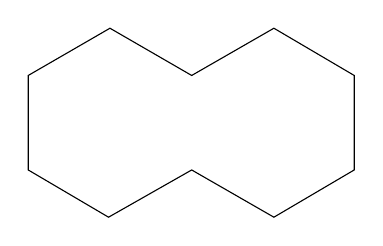
\begin{tikzpicture}[x=1cm,y=1cm, scale=0.6]
  \draw (3.,5.) -- (3.,3.) -- (4.7,2.) -- (6.46,3.) -- (8.2,2.) -- (9.9,3.) -- (9.9,5.) -- (8.2,6.)       -- (6.46,5.) -- (4.73,6.) -- cycle;
  \end{tikzpicture}
\end{center}  

  \item     Pinte metade da figura de forma diferente da do item anterior. 
\begin{center}  
  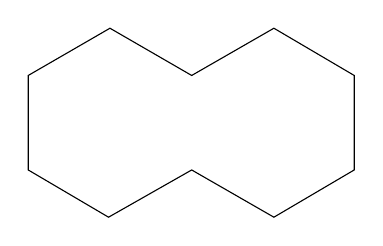
\begin{tikzpicture}[x=1cm,y=1cm, scale=0.6]
  \draw (3.,5.) -- (3.,3.) -- (4.7,2.) -- (6.46,3.) -- (8.2,2.) -- (9.9,3.) -- (9.9,5.) -- (8.2,6.)       -- (6.46,5.) -- (4.73,6.) -- cycle;
  \end{tikzpicture}
\end{center}  

  \item     Pinte a metade da figura de forma diferente das dos dois itens anteriores.     
\begin{center}  
  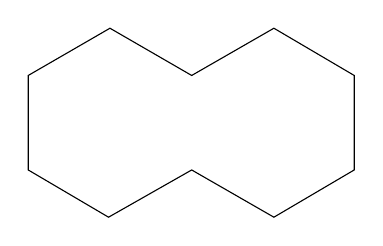
\begin{tikzpicture}[x=1cm,y=1cm, scale=0.6]
  \draw (3.,5.) -- (3.,3.) -- (4.7,2.) -- (6.46,3.) -- (8.2,2.) -- (9.9,3.) -- (9.9,5.) -- (8.2,6.)       -- (6.46,5.) -- (4.73,6.) -- cycle;
  \end{tikzpicture}
\end{center}  
  
  
\end{enumerate} %d


\subsection{Atividade}

Identique as figuras em que a parte pintada é a metade da figura.

\begin{center}
  \begin{tabular}{ccccc} 
%retângulos

\begin{tikzpicture}[scale=5]
 \draw[fill=common] (0,0) rectangle (3,2);
 \draw (3,0) rectangle (6,2); 
 \node at (3,-1) {Figura 1};
\end{tikzpicture}
&
\quad \quad \quad
&
\begin{tikzpicture}[scale=5]
 \draw (0,0) rectangle (3,2);
 \draw (1,0) -- (1,2);
 \draw (1.5,0) -- (1.5,2);
 \draw (2.2,0) -- (2.2,2);
 \draw[fill=common] (3,0) rectangle (6,2) (3,-1) node{Figura 2};
\end{tikzpicture}
&
\quad \quad \quad
&

\begin{tikzpicture}[scale=5]
 \draw (0,0) rectangle (3,2);
 \draw (3,0) rectangle (6,2) (3,-1) node{Figura 3};
 \draw[fill=common] (0,2) rectangle (6,1.2);
 \end{tikzpicture}
\\
 % círculos

 \begin{tikzpicture}[scale=5]
 \draw[fill=common] (0,-2) arc (-90:90: 2);
 \draw (0,2) arc (90:270:2) (0,-3) node{Figura 4};
\end{tikzpicture}
&& 

\begin{tikzpicture}[scale=5]
 \draw[fill=common] (45:2) arc (45:225:2);
 \draw (225:2) arc (225:405:2) (0,-3) node{Figura 5};
 \draw (0,0) -- (0,-2);
 \draw (0,0) -- (-30:2);
 \draw (225:2) -- (45:2);
 \end{tikzpicture}

 &&
 \begin{tikzpicture}[scale=5]
 \draw (0,0) circle (2);
 \draw[fill=common] (0,0) -- (2,0) arc (0:90:2) -- cycle; 
 \draw[fill=common] (0,0) -- (-2,0) arc (180:270: 2) -- cycle;
 \node at (0,-3) {Figura 6};
\end{tikzpicture} 
\\
% hexágonos

\begin{tikzpicture}[scale=5]
 \foreach \x in {0,60,...,300}{
 \draw (\x:2) -- (\x +60: 2);}
 \fill[common] (2,0) -- (60:2) -- (300:2);
 \node at (0,-3) {Figura 7};
\end{tikzpicture}
& &

\begin{tikzpicture}[scale=5]
 \foreach \x in {0,60,...,300}{
 \draw (\x:2) -- (\x +60: 2);}
 \fill[common] (60:2) -- (120:2) -- (180:2) -- (240:2) --cycle;
 \draw (0,0) -- (2,0);
 \draw (0,0) -- (300:2) (0,-3) node{Figura 8};
\end{tikzpicture}
&&

\begin{tikzpicture}[scale=5]
 \foreach \x in {0,60,...,300}{
 \draw (\x:2) -- (\x +60: 2);}
 \fill[common] (0:2) -- (60:2) -- (0:0) --cycle;
 \fill[common] (120:2) -- (180:2) -- (0:0) --cycle;
 \fill[common] (240:2) -- (300:2) -- (0:0) --cycle;
 \node at (0,-3) {Figura 9};
\end{tikzpicture}
\\
%círculo

\begin{tikzpicture}[scale=5]
 \draw[fill=common] (0:2) arc (0:270:2) -- (0,0) -- cycle;
 \draw (270:2) arc (270:360:2);
 \draw (0,0) -- (0,-2);
 \draw (0,0) -- (2,0)  (0,-3) node{Figura 10};
 \end{tikzpicture}
&&
%hexágonos

\begin{tikzpicture}[scale=5]
 \foreach \x in {0,60,...,300}{
 \draw (\x:2) -- (\x +60: 2);}
\fill[common] (120:2) -- (180:2) -- (240:2) -- cycle;
\fill[common] (240:2) -- (300:2) -- (60:2) -- cycle;
 \node at (0,-3) {Figura 11};
\end{tikzpicture}
&&
%retângulo
\begin{tikzpicture}[scale=5]
 \fill[common] (1,-1) rectangle (4,1);
 \draw (0,-1) rectangle (6,1);
 \node at (3,-2) {Figura 12};
 \end{tikzpicture}

\end{tabular}
\end{center}


\subsection{Atividade}







Nas figuras a seguir, um mesmo círculo aparece diferentemente dividido em partes iguais. 
\begin{enumerate} [\quad a)] %s
  \item     Complete as sentenças a seguir identificando os círculos que as tornam verdadeiras.     
\begin{enumerate} [\quad I)] %d
      \item        	A parte colorida do círculo na figura \begin{tikzpicture} \draw (0,0) -- (9,0);\end{tikzpicture} é um quinto do círculo.
      \item        	A parte colorida do círculo na figura \begin{tikzpicture} \draw (0,0) -- (9,0);\end{tikzpicture} é a sexta parte do círculo.
      \item        	A parte colorida do círculo na figura \begin{tikzpicture} \draw (0,0) -- (9,0);\end{tikzpicture} é um sétimo do círculo.
      \item        	A parte colorida do círculo na figura \begin{tikzpicture} \draw (0,0) -- (9,0);\end{tikzpicture} é um oitavo do círculo.
      \item        	A parte colorida do círculo na figura \begin{tikzpicture} \draw (0,0) -- (9,0);\end{tikzpicture} é a nona parte do círculo.
      \item        	A parte colorida do círculo na figura \begin{tikzpicture} \draw (0,0) -- (9,0);\end{tikzpicture} é um décimo do círculo.
\end{enumerate} %d


\hspace{-1cm} \begin{tabular*}{\textwidth}{ccccc}
  
\begin{tikzpicture}[x=1mm,y=1mm, scale=0.6]
      \draw[common,fill] (0,0)
        -- ({7 * 360/9}:20) arc ({7 * 360/9}:{8 * 360/9}:20) -- (0,0);
	  \foreach \x in {1,...,9}
    	{ \draw (0,0) -- ++({360 * \x / 9}:20); }
	  \draw (0,0) circle (20);    
	  \node at (-20,16) {A)};
\end{tikzpicture}

&

\begin{tikzpicture}[x=1mm,y=1mm, scale=0.6]
      \draw[common,fill] (0,0)
        -- ({3 * 360/8}:20) arc ({3 * 360/8}:{4 * 360/8}:20) -- (0,0);
	  \foreach \x in {1,...,8}
    	{ \draw (0,0) -- ++({360 * \x / 8}:20); }
	  \draw (0,0) circle (20);
	  \node at (-20,16) {B)};
\end{tikzpicture}

&
%C)

\begin{tikzpicture}[x=1mm,y=1mm, scale=0.6]
	  \draw[fill=common] (0,0) circle (20);    
	  \node at (-20,16) {C)};
\end{tikzpicture}

&
%D)
\begin{tikzpicture}[x=1mm,y=1mm, scale=0.6]
      \draw[common,fill] (0,0)
        -- ({1.5 * 360/6}:20) arc ({1.5 * 360/6}:{2.5 * 360/6}:20) -- (0,0);
	  \foreach \x in {1.5,...,6.5}
    	{ \draw (0,0) -- ++({360 * \x / 6}:20); }
	  \draw (0,0) circle (20);
	  \node at (-20,16) {D)};
\end{tikzpicture}
&
%E)
\begin{tikzpicture}[x=1mm,y=1mm, scale=0.6]
      \draw[common,fill] (0,0)
        -- (90 :20) arc (90:210:20) -- (0,0);
	  \foreach \x in {1,...,3}
    	{ \draw (0,0) -- ++({90 + 360 * \x / 3}:20); }
	  \draw (0,0) circle (20);
	  \node at (-20,16) {E)};
\end{tikzpicture}
\\
%F)
\begin{tikzpicture}[x=1mm,y=1mm, scale=0.6]
      \draw[common,fill] (0,0)
        -- ({10 + 5 * 360/10}:20) arc ({10 + 5 * 360/10}:{10+6 * 360/10}:20) -- (0,0);
	  \foreach \x in {1,...,10}
    	{ \draw (0,0) -- ++({10 + 360 * \x / 10}:20); }
	  \draw (0,0) circle (20);    
	  \node at (-20,16) {F)};
\end{tikzpicture}
&

%G)
\begin{tikzpicture}[x=1mm,y=1mm, scale=0.6]
      \draw[common,fill] (0,0)-- ({90- 360/5}:20) arc ({90- 360/5}:90:20) -- (0,0);
	  \foreach \x in {1,...,5}
    	{ \draw (0,0) -- ++({90 + 360 * \x / 5}:20); }
	  \draw (0,0) circle (20);    
	  \node at (-20,16) {G)};
\end{tikzpicture}
&
%H)
\begin{tikzpicture}[x=1mm,y=1mm, scale=0.6]
      \draw[common,fill] (0,0)-- (90:20) arc (90:-90:20) -- (0,0);
      \draw (0,0)-- (90:20) arc (90:270:20) -- (0,0);
      \node at (-20,16) {H)};
\end{tikzpicture}
&
%I)
\begin{tikzpicture}[x=1mm,y=1mm, scale=0.6]
      \draw[common,fill] (0,0)-- ({- 360/7}:20) arc ({- 360/7}:{-2 * 360/7}:20) -- (0,0);
	  \foreach \x in {1,...,7}
    	{ \draw (0,0) -- ++({360 * \x / 7}:20); }
	  \draw (0,0) circle (20);    
	  \node at (-20,16) {I)};
\end{tikzpicture}
&
%J)
\begin{tikzpicture}[x=1mm,y=1mm, scale=0.6]
      \draw[common,fill] (0,0)-- (0:20) arc (0:{- 360/4}:20) -- (0,0);
	  \foreach \x in {1,...,4}
    	{ \draw (0,0) -- ++({360 * \x / 4}:20); }
	  \draw (0,0) circle (20);    
	  \node at (-20,16) {J)};
\end{tikzpicture}

 \end{tabular*}


  \item     Dentre as frações do círculo apresentadas, identifique uma que seja menor do que um sexto do círculo.
  \item     Dentre as frações do círculo apresentadas, identifique uma que seja maior do que um nono do círculo.
  \item     Identifique uma fração do círculo que seja menor do que um sexto e maior do que um nono do círculo.
\end{enumerate} %s

\subsection{Atividade}

Em cada uma das imagens, a parte colorida é uma fração da figura. Essas frações podem ser ``um meio'', ``um quarto'' ou ``um décimo'' da figura. Associe cada imagem à fração correspondente.

\begin{center}
\begin{tabular*}{\textwidth}{lcccc}
a)
\begin{tikzpicture}[scale=5]
 \draw (0,0) rectangle (4,2);
 \fill[common] (0,0) -- (4,2) -- (4,0) -- cycle;
\end{tikzpicture}

& \quad \quad \quad &
b)
\begin{tikzpicture}[scale=5]
 \draw (0,0) rectangle (4,2);
 \foreach \n in {0.4,0.8,1.2,...,3.2,3.6}{
 \draw (\n,0) -- (\n,2);}
 \fill[common] (0.8,0) -- (0.8,2) -- (1.2,2) -- (1.2,0) -- cycle;
\end{tikzpicture}
& \quad \quad \quad &

c)
\begin{tikzpicture}[scale=5]
 \draw (0,0) rectangle (4,2);
 \fill[common] (2,1) rectangle (4,2);
 \draw (0,1) -- (4,1);
 \draw (2,0) -- (2,2);
 \end{tikzpicture}
\\

d)
\begin{tikzpicture}[scale=5]
 \fill[common] (45:2) arc (45:135:2) -- (0,0) -- cycle;
 \draw (135:2) arc (135:405:2);
\end{tikzpicture}
& & 
e)
\begin{tikzpicture}[scale=5]
 \foreach \x in {0,60,...,300}{
 \draw (\x:2) -- (\x +60: 2);}
\fill[common] (-2,0) -- (0,0) -- (0,1.73) -- (120:2) -- cycle;
\end{tikzpicture}
& &
f)
\begin{tikzpicture}[scale=5]
 \draw (0,0) rectangle (5,1);
 \draw[fill=common] (0,1) rectangle (5,2);
\end{tikzpicture}
\\
g)
\begin{tikzpicture}[scale=5]
 \draw[fill=common] (0,0) rectangle (2,1);
 \draw (0,1) rectangle (2,3);
\end{tikzpicture} 
& &
h)
\begin{tikzpicture}[scale=5]
 \draw[fill=common] (200:2) arc (200:236:2) -- (0,0) -- cycle;
 \draw (236:2) arc (236:560:2);
\end{tikzpicture} 
&&
i)
\begin{tikzpicture}[scale=5]
 \draw[line width=2pt] (-1,0) arc (180:270:1);
 \draw (0,-1) arc (270:360:1) -- (1,0) arc (180:0:1);
 \end{tikzpicture}
\\
j)
\begin{tikzpicture}
\tikzset{
  annotated cuboid/.pic={
    \tikzset{%
      every edge quotes/.append style={midway, auto},
      /cuboid/.cd,
      #1
    }
    \draw [every edge/.append style={pic actions, densely dashed, opacity=0}, pic actions]
    (0,0,0) coordinate (o) -- ++(-\cubescale*\cubex,0,0) coordinate (a) -- ++(0,-\cubescale*\cubey,0) coordinate (b) edge coordinate [pos=1] (g) ++(0,0,-\cubescale*\cubez)  -- ++(\cubescale*\cubex,0,0) coordinate (c) -- cycle
    (o) -- ++(0,0,-\cubescale*\cubez) coordinate (d) -- ++(0,-\cubescale*\cubey,0) coordinate (e) edge (g) -- (c) -- cycle
    (o) -- (a) -- ++(0,0,-\cubescale*\cubez) coordinate (f) edge (g) -- (d) -- cycle;
 },
  /cuboid/.search also={/tikz},
  /cuboid/.cd,
  width/.store in=\cubex,
  height/.store in=\cubey,
  depth/.store in=\cubez,
  units/.store in=\cubeunits,
  scale/.store in=\cubescale,
  width=100,
  height=100,
  depth=100,
  units=cm,
  scale=.1,
}
    \pic [fill=common] at (0,0) {annotated cuboid={width=25, height=50, depth=8}};
    \pic [fill=white] at (22.5,0) {annotated cuboid={width=225, height=50, depth=8}};
\end{tikzpicture}
&&

l)
\begin{tikzpicture}[scale=5]
 \draw[fill=common] (0,2) rectangle (2,4);
 \draw (0,0) rectangle (2,2);
 \draw (2,0) rectangle (4,2);
 \draw (2,2) rectangle (4,4);
 \end{tikzpicture} 
&&
m)
\begin{tikzpicture}[scale=5]
 \fill[common] (1,0) rectangle (2,1);
 \fill[common] (3,0) rectangle (4,1);
 \fill[common] (0,1) rectangle (1,2);
 \fill[common] (2,1) rectangle (3,2);
 \fill[common] (1,2) rectangle (2,3);
 \fill[common] (3,2) rectangle (4,3);
 \fill[common] (0,3) rectangle (1,4);
 \draw[fill,common] (2,3) rectangle (3,4);
 \draw (0,0) rectangle (4,4);
\end{tikzpicture}

\end{tabular*}
\end{center}


\end{document}